% Provenance (never printed): see sources/outline_sources.md (Year 1: decay systems K-Ar,
% Rb-Sr, U-Pb and radiocarbon; closure temperature; dating sedimentary sequences with
% volcanic ashes; calibrating the scale). Exercise and problem values in the Book 3
% scratch calculator calc/ch25.py; figures from figdata/bachelor-1/decay_curves.py,
% isochron.py and radiocarbon.py (IntCal20, dataset bachelor-1-intcal20).
% The decay law, half-life and decay constant belong to the physics series (recalled);
% the closed system and the isochron of minerals are Book 2's (g12 age-of-the-earth),
% re-founded here with whole-rock samples and least squares. The concordia diagram and
% thermochronology are the Year 3 volume's: prose pointers only. Mass spectrometry is
% the chemistry series' (recalled). The isochron figure uses an invented rhyolite so that
% the Varden granite of the problem is not solved in the course.
\chapter{Métodos de datación radiométrica}\label{ch:b1:radiometric-methods}

En 2001 un equipo que trabajaba con granos detríticos de circón de Jack Hills, en Australia Occidental, informó de uno que había cristalizado
hace \num[uncertainty-mode=separate]{4404 \pm 8} millones de años. Trabajos posteriores confirmaron la edad de estos granos: son el material más antiguo conocido de cualquier tipo formado en la Tierra, y muestran que una \omterm{def:b1:layered-earth:layers}{corteza} se había formado en unos 160 millones de años desde el nacimiento del Sistema Solar. En el otro extremo de la escala, las edades por argón han situado la extinción al final del Cretácico, hace \qty{66.00}{\Ma}, a menos de \num{32000} años del impacto que se cree la causó. Ambos números proceden de contar átomos: un padre radiactivo que se desintegra a un ritmo conocido, y una hija que se acumula. Este capítulo explica cómo se leen estos relojes, por qué cada uno data un suceso distinto y cómo sujetan el cuadro de
\cref{ch:b1:stratigraphic-scale} a una escala de años.
% ledger: wilde01:4404, uw14:jack-hills, ics:base.Paleogene, renne:kpg

\begin{omfigure}
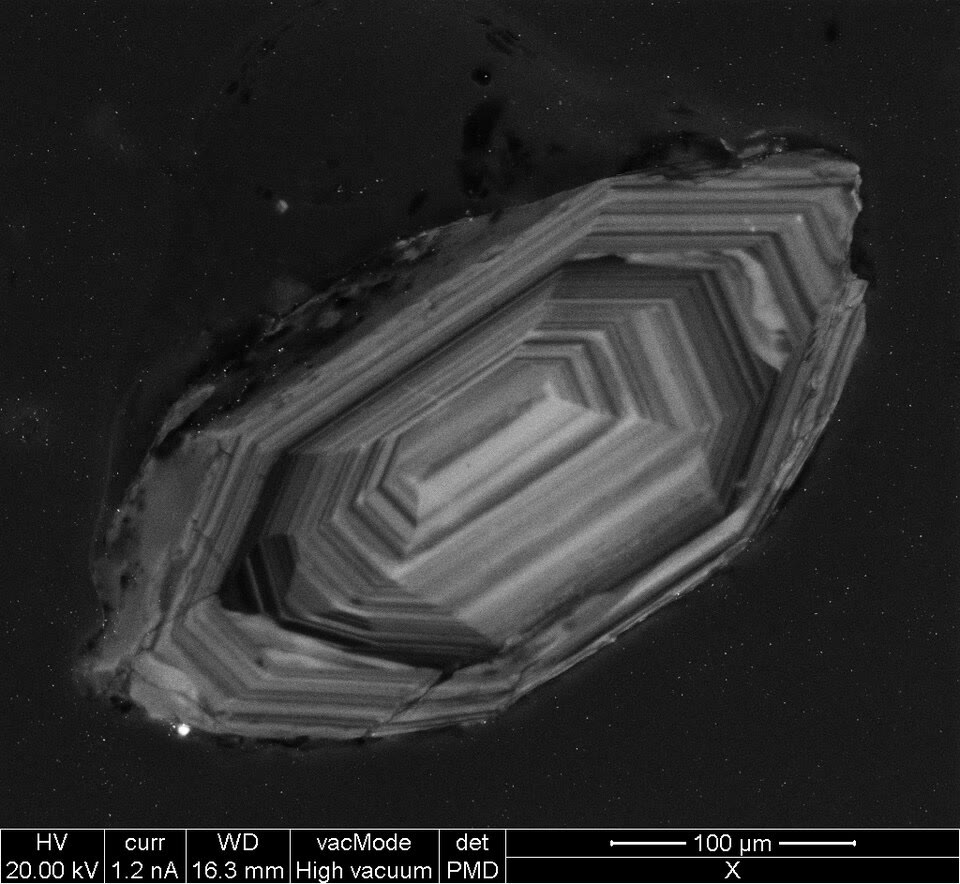
\includegraphics[width=0.5\linewidth]{images/book3/b1-zircon-cl.jpg}

{\small Un grano de circón, de unas tres décimas de milímetro de largo, fotografiado con la luz que emite bajo el haz de electrones de un microscopio electrónico de barrido (catodoluminiscencia). Las bandas que siguen las caras del cristal son zonas de composición ligeramente distinta, depositadas una tras otra a medida que creció. Este grano se extrajo de una arenisca, así que es más antiguo que la arenisca: data la roca de la que fue erosionado. (Emmanuel Roquette, CC~BY-SA~4.0, vía Wikimedia Commons.)}
\label{fig:b1:radiometric-methods:zircon}
\end{omfigure}
% ledger: commons:zircon-cl

\begin{recall}
Los libros de física describen la desintegración radiactiva: los núcleos de un isótopo radiactivo se desintegran al azar, de forma independiente de la temperatura y la presión, de modo que el número $N$ que queda tras un tiempo $t$ sigue $N = N_0\,e^{-\lambda t}$, donde
$\lambda$ es la constante de desintegración; la semivida es $T = \ln 2/\lambda$. Los isótopos de un elemento tienen el mismo número de protones y distinto número de neutrones; los libros de química describen el espectrómetro de masas, que ordena los iones por masa. En el libro 2, año 12, una roca o un \omterm{def:b1:rock-forming-minerals:mineral}{mineral} que no ha intercambiado átomos padre ni hija con su entorno es un sistema cerrado, y los \omterm{def:b1:rock-forming-minerals:mineral}{minerales} del granito de Varden, representados en una \omterm{def:b1:radiometric-methods:isochron}{isócrona} rubidio--estroncio, dieron una edad de 310 millones de años. La biotita, la moscovita y la hornblenda son las \omterm{def:b1:rock-forming-minerals:groups}{micas} y el \omterm{def:b1:rock-forming-minerals:groups}{anfíbol} de \cref{def:b1:rock-forming-minerals:groups}. Una edad entre dos niveles datados puede interpolarse (\cref{prop:b1:stratigraphic-scale:interpolation}).
\end{recall}
% ledger: tulane:radiometric, villa22:rb87

\section{Sistemas de desintegración}\label{sec:b1:radiometric-methods:systems}

Un reloj necesita dos cuentas: lo que queda del padre, y cuánta hija ha producido desde que empezó el reloj.

\begin{definition}[Isótopo padre e hija radiogénica]\label{def:b1:radiometric-methods:radiogenic}
En un sistema de desintegración usado para datar, el \emph{isótopo padre}\index{isótopo padre} es el isótopo radiactivo cuya desintegración sirve de reloj, y la hija es el isótopo que produce esa desintegración. La \emph{hija
radiogénica}\index{hija radiogénica}, escrita $D^*$, es la parte de la hija producida por la desintegración del padre dentro de la muestra desde que empezó el reloj; el resto, $D_0$, estaba allí desde el principio. El número de átomos de la hija medido hoy es $D = D_0 + D^*$.
\end{definition}

\begin{proposition}[Crecimiento radiogénico y ecuación de la edad]\label{prop:b1:radiometric-methods:growth}
En un sistema cerrado que contiene hoy $P$ átomos del padre, la \omterm{def:b1:radiometric-methods:radiogenic}{hija radiogénica} producida en un tiempo $t$ es
\[
  D^* = P\,\bigl(e^{\lambda t} - 1\bigr),
\]
siempre que cada desintegración dé un átomo de la hija. La edad es entonces
\[
  t = \frac{1}{\lambda}\,\ln\!\left(1 + \frac{D^*}{P}\right).
\]
\end{proposition}

\begin{proof}
Por la ley de desintegración, el padre sumaba $P_0 = P\,e^{\lambda t}$ cuando empezó el reloj. En un sistema cerrado, cada átomo de padre que falta se ha
convertido en un átomo de hija, así que $D^* = P_0 - P = P\,(e^{\lambda t} - 1)$. Entonces $e^{\lambda t} = 1 +
D^*/P$; tomando logaritmos se obtiene la edad.
\end{proof}

La edad depende solo de un cociente entre dos números de átomos, que es lo que mejor mide un espectrómetro de masas. La figura siguiente muestra los dos recuentos en unidades de la semivida: tras una semivida $D^*/P = 1$, tras dos $3$, tras tres $7$
--- en general $2^n - 1$ tras $n$ semividas.

\begin{omfigure}
\begin{tikzpicture}
\begin{axis}[omrecord, width=0.72\linewidth, height=5.6cm, xmin=0, xmax=5, ymin=0, ymax=1.05,
  xlabel={tiempo (semividas)}, ylabel={fracción del padre inicial},
  xtick={0,1,...,5}, ytick={0,0.25,0.5,0.75,1}]
% computed in figdata/bachelor-1/decay_curves.py (no real-world number)
\addplot[omThm, line width=1pt] table[x=n, y=P] {figdata/out/bachelor-1-decay_curves-curves.dat};
\addplot[omDef, line width=1pt] table[x=n, y=D] {figdata/out/bachelor-1-decay_curves-curves.dat};
\addplot[only marks, mark=*, mark size=1.4pt, black!60] table[x=n, y=P] {figdata/out/bachelor-1-decay_curves-marks.dat};
\addplot[only marks, mark=*, mark size=1.4pt, black!60] table[x=n, y=D] {figdata/out/bachelor-1-decay_curves-marks.dat};
\node[font=\small, text=omThm, anchor=south west] at (axis cs:0.35,0.80) {padre $P$};
\node[font=\small, text=omDef, anchor=north west] at (axis cs:2.55,0.66) {hija radiogénica $D^*$};
\node[font=\scriptsize, anchor=west, inner sep=1pt] (r1) at (axis cs:0.12,0.5) {$D^*/P = 1$};
\draw[black!60, line width=0.4pt] (r1.east) -- (axis cs:0.95,0.5);
\node[font=\scriptsize, anchor=south] at (axis cs:2,0.77) {$3$};
\node[font=\scriptsize, anchor=south] at (axis cs:3,0.89) {$7$};
\node[font=\scriptsize, anchor=north] at (axis cs:4,0.915) {$15$};
\node[font=\scriptsize, anchor=north east] at (axis cs:4.97,0.95) {$31$};
\end{axis}
\end{tikzpicture}

{\small El padre y su \omterm{def:b1:radiometric-methods:radiogenic}{hija radiogénica} en un sistema cerrado, como fracciones del número inicial de átomos del padre, frente al tiempo contado en semividas. Su suma
se mantiene igual a uno; el cociente $D^*/P$, impreso en cada semivida entera, se duplica y suma uno en cada paso.}
\label{fig:b1:radiometric-methods:decay}
\end{omfigure}

Un reloj solo lee bien dentro de una ventana de edades. Mucho antes de una semivida la hija es una fracción diminuta del padre; tras muchas semividas queda muy poco padre para medir. La tabla siguiente recoge los sistemas más usados, con el material al que se aplica cada uno.

\begin{table}[ht]
\centering
\small
\renewcommand{\arraystretch}{1.25}
\begin{tabular}{|l|l|c|c|>{\raggedright\arraybackslash}p{4.3cm}|}
\hline
padre & hija & semivida (años) & $\lambda$ (por año) & material datado \\
\hline
$^{14}\mathrm{C}$ & $^{14}\mathrm{N}$ & \num{5700} & \num{1.216e-4} & madera, carbón vegetal, hueso, concha \\
$^{40}\mathrm{K}$ & $^{40}\mathrm{Ar}$, $^{40}\mathrm{Ca}$ & \num{1.25e9} & \num{5.543e-10} & \omterm{def:b1:rock-forming-minerals:mineral}{minerales} ricos en potasio: sanidina, biotita, hornblenda \\
$^{87}\mathrm{Rb}$ & $^{87}\mathrm{Sr}$ & \num{4.96e10} & \num{1.3972e-11} & granitos (roca total), \omterm{def:b1:rock-forming-minerals:groups}{micas} \\
$^{147}\mathrm{Sm}$ & $^{143}\mathrm{Nd}$ & \num{1.07e11} & \num{6.46e-12} & rocas y sus \omterm{def:b1:rock-forming-minerals:mineral}{minerales} (\omterm{def:b1:radiometric-methods:isochron}{isócronas}) \\
$^{235}\mathrm{U}$ & $^{207}\mathrm{Pb}$ & \num{7.04e8} & \num{9.8485e-10} & circón \\
$^{238}\mathrm{U}$ & $^{206}\mathrm{Pb}$ & \num{4.47e9} & \num{1.55125e-10} & circón \\
\hline
\end{tabular}
\caption{Los principales sistemas de desintegración. Las constantes de desintegración del potasio-40 y de los dos uranios son los valores convencionales usados para calcular edades; las del rubidio-87 y el samario-147 se calculan a partir de sus semividas, y la del carbono-14 a partir de su semivida de \num{5700} años.}
\label{tab:b1:radiometric-methods:systems}
\end{table}
% ledger: iaea:c14, iaea:k40-branches, amherst:constants, villa22:rb87, iaea:sm147, iaea:isotopes, tulane:kar, tulane:upb-zircon, tulane:c14

Hay dos juegos de números en uso para los mismos núcleos, y una edad debe indicar cuál usó. Las tablas de datos nucleares dan al potasio-40 una semivida de
\num{1.248e9} años y envían \qty{10.72}{\percent} de sus desintegraciones al argón; las constantes usadas por convención en geocronología dan $\lambda = \num{5.543e-10}$ por año (una semivida de \num{1.2505e9}
años) y envían $0.581/5.543 = \qty{10.48}{\percent}$ de las desintegraciones al argón.
Las edades por radiocarbono, como explica \cref{sec:b1:radiometric-methods:kar}, se
calculan con una semivida de \num{5568} años que se sabe demasiado corta. Las
diferencias alcanzan unos pocos por ciento, muy por encima del \qty{0.01}{\percent} con que se citan hoy las mejores edades
(\cref{sec:b1:radiometric-methods:sediments}). La incertidumbre de las constantes de desintegración del propio potasio-40, un núcleo con dos ramas y una semivida larga, limita la exactitud de sus edades.
% ledger: iaea:k40-branches, amherst:constants, sp77:conventional-age, ics:base.Triassic, nmgrl:arar

\begin{proposition}[Precisión de una edad]\label{prop:b1:radiometric-methods:precision}
Si el cociente $R = D^*/P$ se mide con la incertidumbre típica $\sigma_R$,
la edad lleva la incertidumbre
\[
  \sigma_t = \frac{\sigma_R}{\lambda\,(1 + R)}.
\]
\end{proposition}

\begin{proof}
Para un error pequeño $\delta R$, la edad $t = \ln(1+R)/\lambda$ cambia en
$\delta t = t'(R)\,\delta R = \delta R/\bigl(\lambda(1 + R)\bigr)$.
\end{proof}

En una muestra joven, $R$ es pequeño y $\sigma_t \approx \sigma_R/\lambda$: el error absoluto de la edad lo fija lo bien que puede medirse una pequeña cantidad de hija.
Una semivida larga ($\lambda$ pequeño) lo amplifica. Por eso el rubidio--estroncio y el uranio--plomo sirven para rocas de más de unos diez millones de años, mientras que el potasio--argón llega a rocas tan jóvenes como unos diez mil años, y el radiocarbono cubre los últimos \num{70000} años.
% ledger: tulane:ranges

\section{Isócronas}\label{sec:b1:radiometric-methods:isochrons}

La ecuación de la edad necesita $D^*$, pero el instrumento mide $D = D_0 + D^*$, y
$D_0$ rara vez es cero: el estroncio-87 está presente en todo \omterm{def:b1:rock-forming-minerals:mineral}{mineral} que incorporó estroncio al formarse. La \omterm{def:b1:radiometric-methods:isochron}{isócrona} elimina $D_0$ midiendo varias
muestras que empezaron con la misma composición isotópica del elemento hijo.

\begin{definition}[Isócrona, cociente inicial]\label{def:b1:radiometric-methods:isochron}
Sea $S$ un isótopo estable del elemento hijo que ninguna desintegración produce
($^{86}\mathrm{Sr}$ para el estroncio, $^{144}\mathrm{Nd}$ para el neodimio). Una
\emph{isócrona}\index{isócrona} es la recta sobre la que se sitúan, en un gráfico de $y = D/S$ frente a $x = P/S$, las muestras que se formaron a la vez con el mismo valor de $D/S$ y han sido sistemas cerrados desde entonces. Ese valor inicial común
$y_0 = (D/S)_0$ es el \emph{cociente inicial}\index{cociente inicial}.
\end{definition}
% ledger: tulane:radiometric, tulane:c14

\begin{theorem}[La isócrona]\label{thm:b1:radiometric-methods:isochron}
Las muestras que se formaron a la vez con el mismo \omterm{def:b1:radiometric-methods:isochron}{cociente inicial} $y_0$, y han sido sistemas cerrados durante un tiempo $t$,
cumplen
\[
  y = y_0 + \bigl(e^{\lambda t} - 1\bigr)\,x .
\]
Sus puntos están sobre una recta de pendiente $m = e^{\lambda t} - 1$ y ordenada en el origen $y_0$, y $t = \ln(1+m)/\lambda$.
\end{theorem}

\begin{proof}
Para cada muestra, $D = D_0 + P\,(e^{\lambda t} - 1)$ por
\cref{prop:b1:radiometric-methods:growth}. El número de átomos de $S$ no ha cambiado, pues $S$ es estable, no lo produce ninguna desintegración y el sistema es cerrado;
al dividir entre él se obtiene $y = y_0 + (e^{\lambda t} - 1)\,x$, con $y_0$ igual para todas las muestras por hipótesis.
\end{proof}

Cuando cristalizó un granito, todas sus muestras tenían el mismo $y_0$ y se situaban sobre una recta horizontal; cada una ha subido desde entonces en proporción a su $x$, y la recta ha girado en torno a su ordenada en el origen. Las muestras necesitan valores distintos de $x$ para
fijar bien la pendiente: \omterm{def:b1:rock-forming-minerals:mineral}{minerales} con mucho y con poco rubidio, como en el libro 2, o muestras de roca total tomadas de partes más y menos evolucionadas de un mismo cuerpo intrusivo. Un punto fuera de la recta marca una muestra que no fue cerrada, o que no compartía el \omterm{def:b1:radiometric-methods:isochron}{cociente inicial}. El \omterm{def:b1:radiometric-methods:isochron}{cociente inicial} es también un trazador: un magma procedente del \omterm{def:b1:layered-earth:layers}{manto} hereda un $^{87}\mathrm{Sr}/^{86}\mathrm{Sr}$ bajo, de unos $0.7025$, y uno formado por fusión de \omterm{def:b1:layered-earth:layers}{corteza} continental uno alto, de unos $0.710$, porque la \omterm{def:b1:layered-earth:layers}{corteza} es rica en rubidio y ha producido más estroncio-87 a lo largo de los tiempos.
% ledger: tulane:radiometric, tulane:sr-initial

Los puntos reales nunca caen exactamente sobre una recta. La estimación habitual de la recta es la que hace lo más pequeñas posible las distancias verticales al cuadrado de los puntos a ella.

\begin{proposition}[La recta de mínimos cuadrados]\label{prop:b1:radiometric-methods:lsq}
Sean $(x_i, y_i)$, $i = 1, \dots, n$, puntos con al menos dos $x_i$ distintos, de medias $\bar x$ e $\bar y$, y sea
\[
  S_{xx} = \sum_i (x_i - \bar x)^2, \qquad S_{xy} = \sum_i (x_i - \bar x)(y_i - \bar y).
\]
La recta $y = b + m x$ que minimiza $Q(b, m) = \sum_i (y_i - b - m x_i)^2$ tiene
\[
  m = \frac{S_{xy}}{S_{xx}}, \qquad b = \bar y - m\,\bar x ,
\]
y pasa por el centroide $(\bar x, \bar y)$.
\end{proposition}

\begin{proof}
$Q$ es una suma de cuadrados, un polinomio de grado dos en $(b, m)$ que tiende a
infinito en todas las direcciones, así que alcanza su mínimo donde se anulan ambas
derivadas parciales. $\partial Q/\partial b = -2 \sum_i (y_i - b - m x_i) = 0$
da $n\bar y = n b + n m \bar x$, así que $b = \bar y - m \bar x$: la recta pasa
por el centroide. Sustituyendo, $y_i - b - m x_i = (y_i - \bar y) - m(x_i -
\bar x)$, y $\partial Q/\partial m = -2 \sum_i x_i \bigl[(y_i - \bar y) - m(x_i
- \bar x)\bigr] = 0$. Como $\sum_i (y_i - \bar y) = \sum_i (x_i - \bar x) = 0$, $x_i$
puede sustituirse por $x_i - \bar x$ en esta suma, lo que da $S_{xy} - m S_{xx} = 0$.
$S_{xx} > 0$ porque los $x_i$ no son todos iguales.
\end{proof}

La dispersión de los puntos alrededor de la recta da la incertidumbre de la pendiente.
Con los residuos $r_i = y_i - b - m x_i$, la desviación típica de la dispersión es
$s = \sqrt{\sum_i r_i^2/(n-2)}$ --- se usan dos grados de libertad en los dos parámetros ---, y las
incertidumbres típicas de la pendiente y de la ordenada en el origen son
\[
  \sigma_m = \frac{s}{\sqrt{S_{xx}}}, \qquad
  \sigma_b = s\,\sqrt{\frac1n + \frac{\bar x^2}{S_{xx}}} .
\]
Estos dos resultados de estadística se admiten aquí; la edad lleva entonces
$\sigma_t = \sigma_m/\bigl(\lambda(1 + m)\bigr)$, por el mismo argumento de
\cref{prop:b1:radiometric-methods:precision}. Muestran qué hace buena a una \omterm{def:b1:radiometric-methods:isochron}{isócrona}: muchos puntos, repartidos en $x$ (un $S_{xx}$ grande), con poca
dispersión.

\begin{method}[Ajuste de una isócrona]\label{met:b1:radiometric-methods:isochron}
\begin{enumerate}
  \item Medir $x = P/S$ e $y = D/S$ en al menos cuatro muestras de un mismo cuerpo,
        elegidas para repartir $x$ lo más posible.
  \item Representarlas; apartar, con una razón, cualquier punto claramente alejado de la tendencia.
  \item Calcular $\bar x$, $\bar y$, $S_{xx}$, $S_{xy}$, y luego $m = S_{xy}/S_{xx}$
        y $b = \bar y - m \bar x$.
  \item Calcular los residuos, $s$, $\sigma_m$ y $\sigma_b$.
  \item La edad es $t = \ln(1+m)/\lambda$, con $\sigma_t =
        \sigma_m/\bigl(\lambda(1+m)\bigr)$; el \omterm{def:b1:radiometric-methods:isochron}{cociente inicial} es $b \pm \sigma_b$.
\end{enumerate}
\end{method}

\begin{example}[Una riolita inventada]\label{ex:b1:radiometric-methods:rhyolite}
Seis muestras de roca total de una serie de lavas riolíticas (datos del ejercicio) dan:
\begin{center}
\small
\begin{tabular}{|l|cccccc|}
\hline
$x = {}^{87}\mathrm{Rb}/^{86}\mathrm{Sr}$ & 1.85 & 4.62 & 9.30 & 14.75 & 21.20 & 27.60 \\
$y = {}^{87}\mathrm{Sr}/^{86}\mathrm{Sr}$ & 0.71732 & 0.73332 & 0.76164 & 0.79420 & 0.83226 & 0.87028 \\
\hline
\end{tabular}
\end{center}
Aquí $\bar x = 13.22$, $\bar y = 0.784837$, $S_{xx} = 491.41$ y
$S_{xy} = 2.92308$, así que $m = 0.0059484$ y $b = 0.70620$. Los residuos dan
$s = 0.00024$, $\sigma_m = \num{1.10e-5}$ y $\sigma_b = 0.00018$. La edad es
$t = \ln(1.0059484)/\num{1.3972e-11} = \qty{424.5}{\Ma}$, con
$\sigma_t = \num{1.10e-5}/(\num{1.3972e-11} \times 1.0059) = \qty{0.8}{\Myr}$:
\qty[uncertainty-mode=separate]{424.5(8)}{\Ma}, \omterm{def:b1:radiometric-methods:isochron}{cociente inicial}
\num[uncertainty-mode=separate]{0.70620(18)} (figura siguiente).
\end{example}
% values: isochron.py (slope 0.005948361, intercept 0.7061993, age 424.4732, sigma 0.7827871); ledger: villa22:rb87

\begin{omfigure}
\begin{tikzpicture}
\begin{axis}[omrecord, width=0.74\linewidth, height=6cm, xmin=0, xmax=30, ymin=0.70, ymax=0.88,
  xlabel={$^{87}\mathrm{Rb}/^{86}\mathrm{Sr}$}, ylabel={$^{87}\mathrm{Sr}/^{86}\mathrm{Sr}$},
  ytick={0.70,0.72,...,0.88},
  y tick label style={/pgf/number format/.cd, fixed, fixed zerofill, precision=2}]
% computed in figdata/bachelor-1/isochron.py (exercise data, invented rhyolite); ledger: villa22:rb87
\addplot[black!60, densely dotted, line width=0.7pt] table[x=x, y=y] {figdata/out/bachelor-1-isochron-initial.dat};
\addplot[omDef, line width=0.9pt] table[x=x, y=y] {figdata/out/bachelor-1-isochron-line.dat};
\addplot[omThm, only marks, mark=*, mark size=2pt] table[x=x, y=y] {figdata/out/bachelor-1-isochron-points.dat};
\node[font=\scriptsize, text=omDef, anchor=south east, align=right] at (axis cs:19,0.83)
  {pendiente de mínimos cuadrados $0.005948$\\ edad \qty[uncertainty-mode=separate]{424.5(8)}{\Ma}};
\node[font=\scriptsize, text=black!70, anchor=south west] at (axis cs:9,0.7068)
  {cociente inicial $0.70620$, cuando se formaron las lavas};
\end{axis}
\end{tikzpicture}

{\small Una \omterm{def:b1:radiometric-methods:isochron}{isócrona} rubidio--estroncio de seis muestras de roca total de una riolita inventada (datos del ejercicio). Los puntos se dispersan ligeramente alrededor de la recta de mínimos cuadrados, que pasa por su centroide; la línea punteada es donde estaban todos cuando se formaron las lavas.}
\label{fig:b1:radiometric-methods:isochron}
\end{omfigure}

\begin{inthelab}[Pesar isótopos]
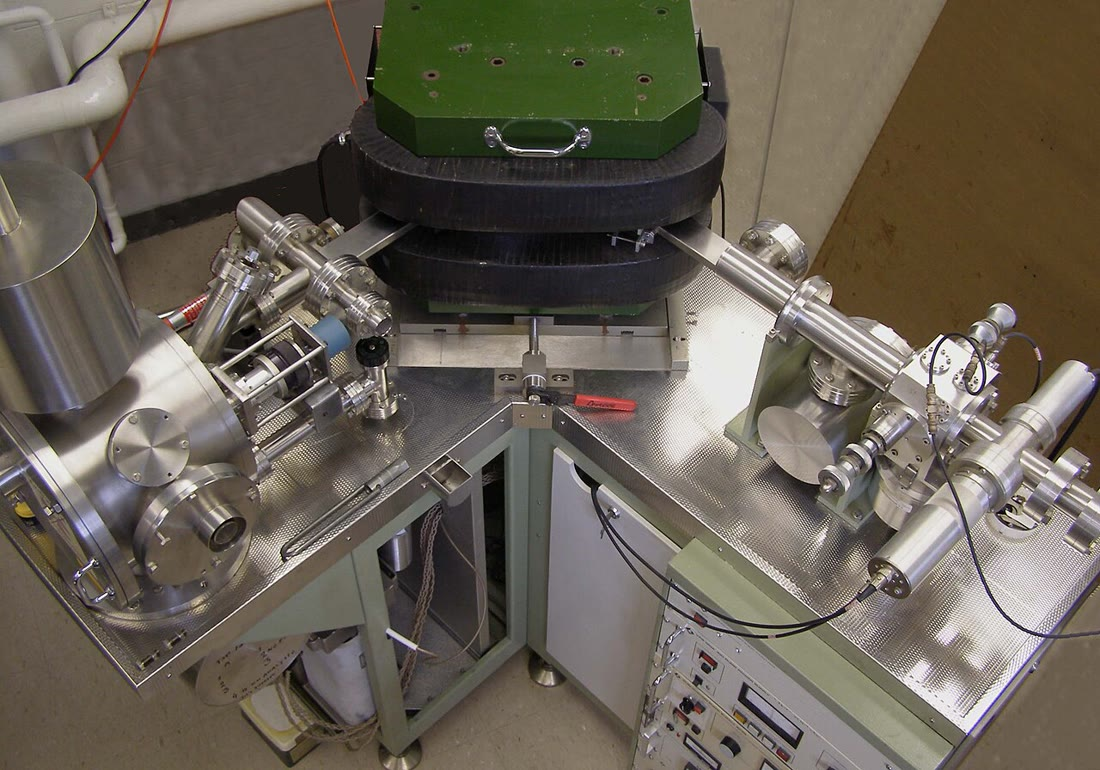
\includegraphics[width=0.42\linewidth]{images/book3/b1-tims.jpg}\hfill
\begin{minipage}[b]{0.55\linewidth}
Un espectrómetro de masas de ionización térmica (izquierda) mide los cocientes isotópicos de elementos como el estroncio. El elemento, separado de la muestra disuelta mediante química, se deposita sobre un filamento metálico en vacío; al calentarlo, emite iones, que se aceleran y se desvían con el campo del gran electroimán (las bobinas negras del centro), los más ligeros más que los pesados, de modo que cada isótopo llega a su propio colector. Los cocientes entre isótopos son lo que el instrumento mide mejor, y por eso los métodos basados solo en cocientes son los más precisos.
(Fotografía: Radiogenic, CC0, vía Wikimedia Commons.)
\end{minipage}
\end{inthelab}
% ledger: commons:tims, amherst:constants

\section{Potasio--argón, uranio--plomo y radiocarbono}\label{sec:b1:radiometric-methods:kar}

\subsection*{Un padre con dos hijas}

\begin{definition}[Desintegración ramificada]\label{def:b1:radiometric-methods:branching}
Un padre sufre una \emph{desintegración ramificada}\index{desintegración ramificada} cuando sus núcleos se desintegran por dos o más vías hacia hijas distintas. Cada vía $i$ tiene su propia
constante de desintegración parcial $\lambda_i$; el padre se desintegra con la constante total
$\lambda = \sum_i \lambda_i$, y una fracción $\lambda_i/\lambda$ de las desintegraciones sigue la vía~$i$. El potasio-40 se desintegra en calcio-40 con $\lambda_\beta =
\num{4.962e-10}$ por año, y en argón-40 con $\lambda_e = \num{0.581e-10}$ por
año.
\end{definition}
% ledger: amherst:constants, iaea:k40-branches

\begin{proposition}[El método de potasio--argón]\label{prop:b1:radiometric-methods:kar}
Un \omterm{def:b1:rock-forming-minerals:mineral}{mineral} que ha conservado todo el argón producido en él, y no contenía ninguno al formarse, contiene tras un tiempo $t$
\[
  {}^{40}\mathrm{Ar}^* = \frac{\lambda_e}{\lambda}\;{}^{40}\mathrm{K}\,\bigl(e^{\lambda t} - 1\bigr),
  \qquad\text{así}\qquad
  t = \frac{1}{\lambda}\,\ln\!\left(1 + \frac{\lambda}{\lambda_e}\,
      \frac{{}^{40}\mathrm{Ar}^*}{{}^{40}\mathrm{K}}\right),
\]
donde ${}^{40}\mathrm{K}$ es el número de átomos de potasio-40 hoy y $\lambda =
\lambda_\beta + \lambda_e$.
\end{proposition}

\begin{proof}
El padre se desintegra con la constante total $\lambda$, sea cual sea la vía, así que por
\cref{prop:b1:radiometric-methods:growth} el número de desintegraciones en el tiempo $t$ es
${}^{40}\mathrm{K}\,(e^{\lambda t} - 1)$. Cada desintegración sigue la vía del argón con
probabilidad $\lambda_e/\lambda$, independientemente de las demás; en el enorme
número de desintegraciones, la fracción que dio argón es $\lambda_e/\lambda$. Esto
da ${}^{40}\mathrm{Ar}^*$; despejando $t$ se obtiene la edad.
\end{proof}

El exponente contiene la constante total, y el factor delante la parcial:
usar $\lambda_e$ en el exponente, como si el argón fuera la única vía, daría una edad
absurdamente errónea. La rama del calcio lleva nueve décimas partes de las desintegraciones, pero no sirve para datar, porque el calcio-40 es el isótopo común de un elemento
abundante en las rocas; el argón, un gas noble, escapa de un fundido, de modo que un cristal
empieza con casi nada. El potasio-40 es \qty{0.0117}{\percent} de los átomos de
potasio. El método necesita las cantidades absolutas de potasio y de argón, medidas por separado. El argón del aire, presente en toda roca, se reconoce por su argón-36 y se resta con el cociente atmosférico
$^{40}\mathrm{Ar}/^{36}\mathrm{Ar} = 295.5$.
% ledger: tulane:kar, iaea:k40-branches, amherst:constants, nmgrl:kar

El método falla de dos maneras. El exceso de argón hace las edades demasiado antiguas: una lava que se enfría deprisa puede atrapar argón del \omterm{def:b1:layered-earth:layers}{manto} en burbujas, y las lavas históricas
suelen dar edades de potasio--argón de 1 a 2 millones de años, un error que solo importa en rocas jóvenes. La pérdida de argón las hace demasiado jóvenes: la mayoría de los \omterm{def:b1:rock-forming-minerals:mineral}{minerales} pierden argón al calentarse por encima de unos \qty{300}{\celsius}, de modo que un metamorfismo posterior reinicia el reloj por completo o en parte, y una pérdida parcial da una edad entre los dos sucesos que no data ninguno de los dos. Se prefieren los \omterm{def:b1:rock-forming-minerals:mineral}{minerales} ricos en potasio: sanidina y biotita, y luego \omterm{def:b1:rock-forming-minerals:groups}{plagioclasa} u hornblenda.
% ledger: tulane:kar, nmgrl:kar

El método argón--argón mide solo cocientes. La muestra se irradia con neutrones rápidos en el núcleo de un reactor nuclear, junto a un \omterm{def:b1:rock-forming-minerals:mineral}{mineral} estándar de edad conocida; la reacción convierte parte de su potasio-39 en argón-39, que hace entonces de representante del potasio, y el estándar da el rendimiento de la reacción. Los dos isótopos se miden juntos en el mismo gas. La muestra puede calentarse después por etapas, con un horno o con un láser; cada etapa da una edad, y las edades se representan frente a la fracción acumulada de argón-39 liberada, un espectro de edades. Las etapas que concuerdan dentro de sus errores forman una meseta; un espectro sin ella advierte de que el \omterm{def:b1:rock-forming-minerals:mineral}{mineral} no se mantuvo cerrado. La sincronía del impacto y de la extinción al final del Cretácico descansa en edades argón--argón.
% ledger: amherst:arar, nmgrl:arar, renne:kpg

\subsection*{Dos relojes de uranio}

El uranio tiene dos isótopos de vida larga, el uranio-238, que se desintegra en plomo-206, y el uranio-235, que lo hace en plomo-207, a ritmos distintos; hoy
$^{235}\mathrm{U}/^{238}\mathrm{U} = 0.0072567$, es decir, un átomo entre 137.8. Un \omterm{def:b1:rock-forming-minerals:mineral}{mineral} con uranio lleva así dos relojes independientes, cada uno con su propia
ecuación de crecimiento, ${}^{206}\mathrm{Pb}^* = {}^{238}\mathrm{U}\,(e^{\lambda_{238} t} - 1)$
y ${}^{207}\mathrm{Pb}^* = {}^{235}\mathrm{U}\,(e^{\lambda_{235} t} - 1)$. Si las dos edades concuerdan, se dice que son concordantes, y la concordancia es una prueba de que el \omterm{def:b1:rock-forming-minerals:mineral}{mineral} se mantuvo cerrado, algo que ningún reloj por sí solo puede aportar. El desacuerdo proviene sobre todo del plomo perdido en partes del cristal dañadas por la radiación
del propio uranio; una gráfica de los dos cocientes uno frente al otro, el diagrama de concordia, recupera entonces tanto la edad del cristal como la del suceso que le hizo perder plomo --- una herramienta del libro de tercer año.
% ledger: amherst:constants, tulane:upb-zircon

Circón, $\mathrm{ZrSiO_4}$, es el \omterm{def:b1:rock-forming-minerals:mineral}{mineral} preferido: incorpora uranio a su estructura pero casi nada de plomo, así que casi todo su plomo es radiogénico; es duro, resiste la meteorización y sobrevive al metamorfismo, de modo que los granos erosionados de una roca conservan su edad en las arenas derivadas de ella. También se usan el apatito y la esfena, con menos frecuencia.
% ledger: tulane:upb-zircon, commons:zircon-cl

\subsection*{Radiocarbono}

El carbono-14 se produce continuamente en la alta atmósfera a partir de nitrógeno-14 bombardeado por rayos cósmicos. Se une al carbono de la atmósfera; los organismos vivos
intercambian carbono con la atmósfera y mantienen su proporción de carbono-14. Al morir cesa el intercambio y el carbono-14 vuelve a desintegrarse en nitrógeno-14. Como la proporción inicial es la de la atmósfera, la edad se deduce de la ley de desintegración sola, sin \omterm{def:b1:radiometric-methods:isochron}{isócrona}: $t = -\tau \ln(A/A_0)$, donde $A$ es la
actividad del carbono de la muestra, $A_0$ la del carbono vivo y $\tau =
1/\lambda$ la vida media. La madera, el carbón vegetal, el hueso, los dientes y la concha se datan así, hasta unas decenas de miles de años: como mucho unos \num{70000} años.
% ledger: tulane:c14, iaea:c14

\begin{definition}[Edad radiocarbónica, curva de calibración]\label{def:b1:radiometric-methods:radiocarbon}
La \emph{edad radiocarbónica}\index{edad radiocarbónica} (convencional) de una muestra es
\[
  t = -8033 \,\ln \frac{A_{\mathrm{SN}}}{A_{\mathrm{ON}}} \ \text{años BP},
\]
donde $A_{\mathrm{SN}}$ es la actividad del carbono de la muestra y
$A_{\mathrm{ON}}$ la del estándar de referencia; usa la semivida de
\num{5568} años (vida media \num{8033} años), normaliza las actividades por el fraccionamiento isotópico del carbono ($\delta^{13}\mathrm{C} = \qty{-25}{\permil}$), y cuenta los años antes de 1950 d.~C. (BP, ``antes del presente''). Una
\emph{curva de calibración}\index{curva de calibración} da la edad radiocarbónica de muestras de edad de calendario conocida; leída al revés, convierte una edad radiocarbónica en un intervalo de edades de calendario (cal BP).
\end{definition}
% ledger: sp77:conventional-age, reimer20:intcal20

La \omterm{def:b1:radiometric-methods:radiocarbon}{edad radiocarbónica} no es una edad en años de calendario, por dos razones. La semivida de \num{5568} años, el valor de Libby, conservado por convención, es más corta que los verdaderos \num{5700} años, así que las \omterm{def:b1:radiometric-methods:radiocarbon}{edades radiocarbónicas} quedan unas
\qty{2.4}{\percent} cortas. Más importante aún, la proporción de carbono-14 en la atmósfera no ha sido constante. La \omterm{def:b1:radiometric-methods:radiocarbon}{curva de calibración} mide ambos efectos a la vez, sobre archivos fechados de forma independiente: anillos de árboles hasta unas
\num{13900} cal BP, y más allá, secuencias flotantes de anillos, sedimentos lacustres y marinos, depósitos de cuevas y corales, hasta \num{55000} cal BP (figura siguiente).
% ledger: sp77:conventional-age, iaea:c14, reimer20:intcal20

\begin{omfigure}
\begin{tikzpicture}
\begin{axis}[name=main, omrecord, width=0.5\linewidth, height=6cm, xmin=0, xmax=12, ymin=0, ymax=12,
  xlabel={edad de calendario (miles cal BP)}, ylabel={edad radiocarbónica (miles BP)},
  xtick={0,2,...,12}, ytick={0,2,...,12}]
% figdata/bachelor-1/radiocarbon.py, IntCal20 (dataset bachelor-1-intcal20); ledger: data:b3-intcal20
\addplot[black!50, dashed, domain=0:12, samples=2] {x};
\addplot[omDef, line width=0.9pt] table[x=cal, y=c14] {figdata/out/bachelor-1-radiocarbon-curve.dat};
\draw[omThm, line width=0.6pt] (axis cs:2.3,2.3) rectangle (axis cs:2.9,2.9);
\node[font=\scriptsize, anchor=east, text=black!60] at (axis cs:8.4,10.4) {edades iguales};
\node[font=\scriptsize, text=omDef, anchor=north west] at (axis cs:7.4,5.6) {IntCal20};
\end{axis}
\begin{axis}[at={(main.east)}, anchor=west, xshift=2.1cm, omrecord, width=0.38\linewidth, height=6cm,
  xmin=2300, xmax=2900, ymin=2300, ymax=2900, xlabel={edad de calendario (cal BP)}, ylabel={edad radiocarbónica (BP)},
  xtick={2300,2500,2700,2900}, ytick={2300,2500,2700,2900},
  x tick label style={/pgf/number format/.cd, set thousands separator={}},
  y tick label style={/pgf/number format/.cd, set thousands separator={}}]
\addplot[name path=hi, draw=none, forget plot] table[x=cal, y=hi] {figdata/out/bachelor-1-radiocarbon-zoom.dat};
\addplot[name path=lo, draw=none, forget plot] table[x=cal, y=lo] {figdata/out/bachelor-1-radiocarbon-zoom.dat};
\addplot[omDef!25, forget plot] fill between[of=hi and lo];
\addplot[omDef, line width=0.8pt] table[x=cal, y=c14] {figdata/out/bachelor-1-radiocarbon-zoom.dat};
\addplot[omThm, line width=0.6pt, domain=2300:2900, samples=2] {2480};
\draw[omThm, densely dotted] (axis cs:2495,2300) -- (axis cs:2495,2480);
\draw[omThm, densely dotted] (axis cs:2699,2300) -- (axis cs:2699,2480);
\node[font=\scriptsize, text=omThm, anchor=south west] at (axis cs:2310,2485) {$2480$ BP};
\end{axis}
\end{tikzpicture}

{\small Izquierda: la \omterm{def:b1:radiometric-methods:radiocarbon}{curva de calibración} IntCal20 de los últimos \num{12000} años, \omterm{def:b1:radiometric-methods:radiocarbon}{edad radiocarbónica} frente a edad de calendario; la línea discontinua marca dónde serían iguales las dos. Derecha: el recuadro de la izquierda ampliado, con la banda de una incertidumbre típica de la curva. Entre \num{2500} y \num{2700} cal BP la curva
es casi plana: una \omterm{def:b1:radiometric-methods:radiocarbon}{edad radiocarbónica} de 2480 años BP corresponde a edades de calendario de unos \num{2495} a \num{2699} cal BP.}
\label{fig:b1:radiometric-methods:intcal}
\end{omfigure}
% ledger: data:b3-intcal20, reimer20:intcal20

A \num{2000} cal BP la curva da \num[uncertainty-mode=separate]{2070 \pm 14} años BP; a
\num{12000} cal BP, \num{10306}: las \omterm{def:b1:radiometric-methods:radiocarbon}{edades radiocarbónicas} allí son \num{1694} años más jóvenes que las edades de calendario, mucho más que el \qty{2.4}{\percent} de la semivida. La curva oscila, y donde es plana una \omterm{def:b1:radiometric-methods:radiocarbon}{edad radiocarbónica} corresponde a un intervalo largo de edades de calendario, por muy precisa que sea la medida.
% ledger: data:b3-intcal20

\begin{dated}{2020}
% ledger: reimer20:intcal20
La curva en uso para el hemisferio norte es IntCal20, publicada en 2020. Sustituyó a IntCal13, añadiendo datos nuevos y extendiendo la curva hasta \num{55000} cal BP,
con curvas separadas para el hemisferio sur y para la superficie del océano. Las \omterm{def:b1:radiometric-methods:radiocarbon}{curvas de calibración} se revisan a medida que se miden nuevos archivos, así que una edad de calendario debe nombrar la curva que la produjo.
\end{dated}

\section{Temperatura de cierre}\label{sec:b1:radiometric-methods:closure}

Un \omterm{def:b1:rock-forming-minerals:mineral}{mineral} que cristaliza de un magma a \qty{800}{\celsius} no inicia su reloj de inmediato. Mientras está caliente, los átomos de la hija --- el argón sobre todo ---
se difunden a través de su red y escapan; solo cuando se ha enfriado lo bastante la difusión se vuelve demasiado lenta para importar, y la hija empieza a acumularse.
% ledger: leeds:closure, tulane:kar, tulane:magma-types

\begin{definition}[Temperatura de cierre, edad de enfriamiento]\label{def:b1:radiometric-methods:closure}
La \emph{temperatura de cierre}\index{temperatura de cierre} de un \omterm{def:b1:rock-forming-minerals:mineral}{mineral} para un sistema de desintegración es la temperatura por debajo de la cual los átomos padre e hija ya no se difunden hacia dentro ni hacia fuera de su red con la rapidez suficiente para importar, de modo que el \omterm{def:b1:rock-forming-minerals:mineral}{mineral} se comporta como un sistema cerrado. Una \emph{edad de enfriamiento}\index{edad de enfriamiento} es una edad medida en un \omterm{def:b1:rock-forming-minerals:mineral}{mineral} que se formó por encima de su temperatura de cierre: data el momento en que el \omterm{def:b1:rock-forming-minerals:mineral}{mineral} se enfrió por debajo de esa temperatura, no el momento en que se formó.
\end{definition}
% ledger: leeds:closure

Las \omterm{def:b1:radiometric-methods:closure}{temperaturas de cierre} difieren según el \omterm{def:b1:rock-forming-minerals:mineral}{mineral}, porque las redes difieren, y según el elemento, porque átomos distintos se difunden a través de una misma red a ritmos distintos
(figura siguiente). Son aproximadas: dos tablas dan \qty{280}{\celsius} y \qty{350}{\celsius} para el argón en la biotita, \qty{530}{\celsius} y \qty{550}{\celsius} para el argón en la hornblenda. Las trazas de fisión, las huellas de daño que deja en un cristal la fisión espontánea de núcleos de uranio, se borran a temperaturas aún más bajas.
% ledger: leeds:closure, amherst:closure

\begin{omfigure}
\begin{tikzpicture}
\begin{axis}[width=0.8\linewidth, height=7cm, xbar, bar width=7pt, xmin=0, xmax=850,
  xlabel={temperatura de cierre (\unit{\celsius})},
  symbolic y coords={zrupb,spupb,hbar,mssr,msar,btsr,btar,zrft,kfsar,apft},
  ytick={zrupb,spupb,hbar,mssr,msar,btsr,btar,zrft,kfsar,apft}, y dir=reverse, enlarge y limits=0.07,
  yticklabels={{circón, U--Pb},{esfena, U--Pb},{hornblenda, K--Ar},{moscovita, Rb--Sr},{moscovita, K--Ar},{biotita, Rb--Sr},{biotita, K--Ar},{circón, trazas de fisión},{feldespato potásico, K--Ar},{apatito, trazas de fisión}},
  y tick label style={font=\scriptsize}, x tick label style={font=\scriptsize},
  axis x line*=bottom, axis y line*=left]
% ledger: leeds:closure (values as tabulated; > lower bound, ~ approximate, ranges and +- as given)
\addplot[fill=omDef!55, draw=omDef, error bars/.cd, x dir=both, x explicit]
  coordinates {(750,zrupb) (650,spupb) (530,hbar) +- (40,0) (500,mssr) (350,msar) (320,btsr)
               (280,btar) +- (40,0) (200,zrft) +- (25,0) (130,kfsar) (105,apft) +- (10,0)};
\node[font=\scriptsize, anchor=west] at (axis cs:755,zrupb) {$> 750$};
\node[font=\scriptsize, anchor=west] at (axis cs:655,spupb) {$> 650$};
\node[font=\scriptsize, anchor=west] at (axis cs:575,hbar) {$530 \pm 40$};
\node[font=\scriptsize, anchor=west] at (axis cs:505,mssr) {$500$};
\node[font=\scriptsize, anchor=west] at (axis cs:355,msar) {$\approx 350$};
\node[font=\scriptsize, anchor=west] at (axis cs:325,btsr) {$320$};
\node[font=\scriptsize, anchor=west] at (axis cs:325,btar) {$280 \pm 40$};
\node[font=\scriptsize, anchor=west] at (axis cs:230,zrft) {$175$--$225$};
\node[font=\scriptsize, anchor=west] at (axis cs:135,kfsar) {$\approx 130$, con pérdidas};
\node[font=\scriptsize, anchor=west] at (axis cs:120,apft) {$105 \pm 10$};
\end{axis}
\end{tikzpicture}

{\small \omterm{def:b1:radiometric-methods:closure}{Temperaturas de cierre} de los principales relojes \omterm{def:b1:rock-forming-minerals:mineral}{minerales}, según una tabla publicada. U--Pb es uranio--plomo, K--Ar potasio--argón (y argón--argón), Rb--Sr
rubidio--estroncio. Para las trazas de fisión, el valor es la temperatura a la que se borran las trazas.}
\label{fig:b1:radiometric-methods:closure}
\end{omfigure}

En un plutón que se enfrió despacio, los relojes se cierran, por tanto, uno tras otro,
del más caliente al más frío: primero el circón, cerca de su cristalización; luego la hornblenda, después la moscovita y la biotita. La dispersión de sus edades registra el enfriamiento.

\begin{proposition}[Velocidad de enfriamiento entre dos cierres]\label{prop:b1:radiometric-methods:cooling}
Si dos \omterm{def:b1:rock-forming-minerals:mineral}{minerales} de una misma roca, de \omterm{def:b1:radiometric-methods:closure}{temperaturas de cierre} $T_1 > T_2$, dan las \omterm{def:b1:radiometric-methods:closure}{edades de enfriamiento} $t_1 > t_2$, la velocidad media de enfriamiento entre los dos cierres es
\[
  \dot T = \frac{T_1 - T_2}{t_1 - t_2}.
\]
Si la roca estaba a una profundidad en la que la temperatura subía con la profundidad a un gradiente constante
$G$ bajo una superficie a la temperatura $T_s$, estaba a la profundidad $z_i
= (T_i - T_s)/G$ cuando cerró el reloj $i$.
\end{proposition}

\begin{proof}
La roca estaba a $T_1$ en el momento $t_1$ y a $T_2$ en el momento $t_2$; la velocidad media de cambio de su temperatura es el cociente de las dos diferencias. Con un
\omterm{def:b1:heat-budget:geotherm}{geotermo} lineal (\cref{def:b1:heat-budget:geotherm}), $T = T_s + G z$, lo que da la profundidad.
\end{proof}

La profundidad da una velocidad de exhumación, una vez que se conoce el momento en que la roca llegó a la superficie, como en el problema de este capítulo. El método es tosco: las \omterm{def:b1:radiometric-methods:closure}{temperaturas de cierre} tienen una incertidumbre de decenas de grados, y se supone que el \omterm{def:b1:heat-budget:geotherm}{geotermo} es constante en el tiempo. La termocronología, la reconstrucción
detallada de las trayectorias temperatura--tiempo a partir de muchos relojes, es materia del libro de tercer año.

\section{Datación de secuencias sedimentarias}\label{sec:b1:radiometric-methods:sediments}

La mayoría de las rocas sedimentarias no pueden datarse directamente. Sus granos son más antiguos que la roca: un circón detrítico, como el grano del principio de este capítulo, data la roca de la que fue erosionado. El radiocarbono solo data materia orgánica joven. Las edades de la
carta proceden, por tanto, de rocas que cristalizaron en el momento en que se depositaron --- cenizas volcánicas y coladas de lava dentro de la secuencia --- y de rocas ígneas que la cortan.
% ledger: tulane:upb-zircon, tulane:c14, commons:zircon-cl

\begin{definition}[Edad de acotación]\label{def:b1:radiometric-methods:bracketing}
Una \emph{edad de acotación}\index{edad de acotación} es un límite impuesto a la edad de un nivel sedimentario por rocas datadas relacionadas con él mediante los principios de la estratigrafía: una edad máxima a partir de una capa datada situada debajo, o del grano detrítico más joven de esa capa; una edad
mínima a partir de una capa datada situada encima, o de una intrusión que lo corta. Un nivel entre un máximo y un mínimo está acotado.
\end{definition}

\begin{omfigure}
\begin{tikzpicture}[x=1cm, y=0.62cm]
  % column
  \fill[lith shale] (0,0) rectangle (2.4,3);
  \fill[lith sandstone] (0,3) rectangle (2.4,6);
  \fill[lith shale] (0,6) rectangle (2.4,9);
  \fill[lith limestone] (0,9) rectangle (2.4,12);
  \draw (0,0) rectangle (2.4,12);
  % ash bed below, lava flow above
  \fill[omThm!70] (0,2.0) rectangle (2.4,2.3);
  \fill[black!65] (0,9.0) rectangle (2.4,9.6);
  % boundary
  \draw[omDef, line width=1.2pt] (-0.3,7.2) -- (2.7,7.2);
  % dyke cutting everything
  \fill[black!40] (1.55,0) -- (1.85,0) -- (1.95,12) -- (1.65,12) -- cycle;
  % detrital zircons
  \foreach \p in {(0.4,3.6),(0.9,4.5),(0.5,5.4),(1.2,3.9),(0.8,5.0)}
    \fill[omThm] \p circle (1.3pt);
  % labels
  \node[anchor=west, font=\small, align=left] at (3.0,2.15) {capa de ceniza, $t_1$: edad máxima};
  \node[anchor=west, font=\small, align=left] at (3.0,4.5) {circón detrítico más joven, $t_0$:\\edad máxima de la arenisca};
  \node[anchor=west, font=\small, text=omDef] at (3.0,7.2) {nivel por datar};
  \node[anchor=west, font=\small, align=left] at (3.0,9.3) {colada de lava, $t_2$: edad mínima};
  \node[anchor=west, font=\small, align=left] at (3.0,11.3) {dique, $t_3$: edad mínima de\\cada capa que corta};
  \draw[black!50] (2.5,2.15) -- (2.95,2.15);
  \draw[black!50] (1.25,4.5) -- (2.95,4.5);
  \draw[black!50] (2.5,9.3) -- (2.95,9.3);
  \draw[black!50] (1.95,11.3) -- (2.95,11.3);
\end{tikzpicture}

{\small Edades que acotan un nivel en una secuencia sedimentaria (esquema). La capa de ceniza inferior y el circón detrítico más joven de la arenisca dan edades máximas; la colada de lava superior y el dique que corta toda la secuencia dan edades mínimas. El nivel es más joven que $t_1$ y más antiguo que $t_2$; el dique añade solo que es más antiguo que $t_3$.}
\label{fig:b1:radiometric-methods:bracketing}
\end{omfigure}

Las mejores acotaciones son cercanas y precisas: dos capas de ceniza a pocos metros una de otra, datadas en circón con una precisión de unas decenas de miles de años, con el nivel entre ellas interpolado mediante
\cref{prop:b1:stratigraphic-scale:interpolation}. En Meishan, el GSSP de la base del Triásico yace entre cinco capas de ceniza datadas; la extinción queda acotada entre \qty[uncertainty-mode=separate]{251.941(37)}{\Ma}
y \qty[uncertainty-mode=separate]{251.880(31)}{\Ma}, y la base del sistema se sitúa en \qty[uncertainty-mode=separate]{251.902(24)}{\Ma}
(\cref{sec:b1:stratigraphic-scale:extinctions}). Las capas de ceniza, llevadas por el viento a través de facies distintas, son a la vez líneas de tiempo y relojes.
% ledger: burgess:end-permian, gssp:induan, ics:base.Triassic

La carta es solo tan precisa como las capas datadas cercanas a cada límite. La base del Triásico se conoce con \qty{0.024}{\Myr} de error, una parte en diez mil; la base del Carbonífero, con \qty{0.19}{\Myr}; la base del Devónico, con
\qty{1.36}{\Myr}. Donde no hay ninguna capa datada cerca de un límite, su edad se interpola entre otras lejanas, y su incertidumbre crece en consecuencia. Cada nueva capa de ceniza datada cerca de un límite puede moverlo, por eso la carta lleva una fecha de versión.
% ledger: ics:base.Triassic, ics:base.Carboniferous, gssp:lochkovian

\section{Ejercicios}

\begin{exercise}[$\star$]\label{exo:b1:radiometric-methods:1}
(a)~Un \omterm{def:b1:rock-forming-minerals:mineral}{mineral} contiene tres veces más átomos de \omterm{def:b1:radiometric-methods:radiogenic}{hija radiogénica} que de padre. ¿Cuántas semividas tiene? (b)~Calcúlese $D^*/P$ tras
\qty{310}{\Myr} para el rubidio-87 y para el uranio-235, con las constantes de
\cref{tab:b1:radiometric-methods:systems}. ¿Qué cociente es más fácil de medir con precisión? (c)~¿Tras cuántas semividas queda menos del \qty{1}{\percent} del padre?
% ledger: villa22:rb87, amherst:constants
\end{exercise}

\begin{exercise}[$\star$]\label{exo:b1:radiometric-methods:2}
¿Qué método de \cref{tab:b1:radiometric-methods:systems} usaría, y sobre qué material, para datar: (a)~carbón vegetal de un hogar de unos \num{8000} años;
(b)~una capa de ceniza que se cree de unos \qty{66}{\Ma}, rica en sanidina y circón; (c)~un granito de unos \qty{2.7}{\Ga}; (d)~una concha de unos
\num{40000} años; (e)~una caliza del Jurásico sin ninguna capa volcánica?
% ledger: tulane:c14, tulane:kar, tulane:upb-zircon
\end{exercise}

\begin{exercise}[$\star$]\label{exo:b1:radiometric-methods:3}
El carbono de un trozo de madera tiene una cuarta parte de la actividad del estándar, tras la normalización. (a)~Calcúlese su \omterm{def:b1:radiometric-methods:radiocarbon}{edad radiocarbónica} convencional. (b)~Calcúlese
su edad con la semivida de \num{5700} años. (c)~¿Por qué ninguna de estas es su edad en años de calendario, y cómo se obtiene esa edad?
% ledger: sp77:conventional-age, iaea:c14
\end{exercise}

\begin{exercise}[$\star$]\label{exo:b1:radiometric-methods:4}
Un granito da una edad uranio--plomo en circón de \qty{420}{\Ma}, una edad potasio--argón en hornblenda de \qty{410}{\Ma} y otra en biotita de
\qty{398}{\Ma}. (a)~¿Por qué las tres edades son distintas, y en este orden? (b)~Con las \omterm{def:b1:radiometric-methods:closure}{temperaturas de cierre} de la figura de
\cref{sec:b1:radiometric-methods:closure}, calcúlese la velocidad media de enfriamiento entre los cierres de la hornblenda y de la biotita. (c)~¿Qué puede decirse de la velocidad de enfriamiento entre el cierre del circón y el de la hornblenda?
% ledger: leeds:closure
\end{exercise}

\begin{exercise}[$\star\star$]\label{exo:b1:radiometric-methods:5}
Cuatro muestras de roca total de un gneis (datos del ejercicio) dan
$^{87}\mathrm{Rb}/^{86}\mathrm{Sr} = 2.0$, $5.0$, $9.0$, $14.0$ y
$^{87}\mathrm{Sr}/^{86}\mathrm{Sr} = 0.7323$, $0.7741$, $0.8307$, $0.9010$.
(a)~Calcúlese la recta de mínimos cuadrados por el método de
\cref{met:b1:radiometric-methods:isochron}. (b)~Calcúlense la edad y el \omterm{def:b1:radiometric-methods:isochron}{cociente inicial}. (c)~Calcúlense $s$ y la incertidumbre de la edad. (d)~¿Apunta el \omterm{def:b1:radiometric-methods:isochron}{cociente inicial} a una fuente en el \omterm{def:b1:layered-earth:layers}{manto} o en la \omterm{def:b1:layered-earth:layers}{corteza}?
% ledger: villa22:rb87, tulane:sr-initial
\end{exercise}

\begin{exercise}[$\star\star$]\label{exo:b1:radiometric-methods:6}
Una sanidina de una capa de ceniza contiene \qty{10.0}{\percent} de potasio en masa y \qty{1.169}{nmol} de argón-40 radiogénico por gramo. (a)~Con la masa atómica del potasio,
\qty{39.098}{g.mol^{-1}}, y la abundancia del potasio-40, calcúlese el número de moles de potasio-40 por gramo. (b)~Calcúlese la edad potasio--argón. (c)~Si se hubiera atrapado el \qty{0.5}{\percent} del argón medido cuando cayó la ceniza, en lugar de producirse por desintegración, ¿en cuánto sería demasiado antigua la edad? ¿Es esto una preocupación aquí?
% ledger: ciaaw:K, iaea:k40-branches, amherst:constants, tulane:kar
\end{exercise}

\begin{exercise}[$\star\star$]\label{exo:b1:radiometric-methods:7}
La curva IntCal20 da las \omterm{def:b1:radiometric-methods:radiocarbon}{edades radiocarbónicas} \num[uncertainty-mode=separate]{2070 \pm 14} años BP a \num{2000}
cal BP, \num{7178} a \num{8000} cal BP y \num{10306} a \num{12000} cal BP.
(a)~Una semilla da \num[uncertainty-mode=separate]{2070 \pm 14} años BP. ¿Cuál es su edad de calendario? (b)~Otra da \num[uncertainty-mode=separate]{2480 \pm 15} años
BP; con el panel de la derecha de la figura de
\cref{sec:b1:radiometric-methods:kar}, calcúlese su intervalo de edades de calendario y explíquese por qué es tan amplio. (c)~¿En cuántos años, y en qué sentido, difieren las \omterm{def:b1:radiometric-methods:radiocarbon}{edades radiocarbónicas} de las edades de calendario a \num{2000}, \num{8000} y \num{12000} cal BP? ¿Crece la diferencia en proporción a la edad?
% ledger: data:b3-intcal20
\end{exercise}

\begin{exercise}[$\star\star$]\label{exo:b1:radiometric-methods:8}
En una sección marina, una capa de ceniza a \qty{4}{m} se data en
\qty[uncertainty-mode=separate]{94.50(10)}{\Ma} y una colada de lava a \qty{20}{m} en \qty[uncertainty-mode=separate]{93.80(12)}{\Ma}; un dique que corta toda la
sección se data en \qty[uncertainty-mode=separate]{93.20(8)}{\Ma}. El circón detrítico más joven de una arenisca a \qtyrange{6}{10}{m} es
\qty[uncertainty-mode=separate]{95.3(4)}{\Ma}. Un límite de \omterm{def:b1:stratigraphic-scale:chronostratigraphy}{piso} se sitúa a \qty{12}{m}. (a)~¿Cuáles de las cuatro edades acotan el límite, y cuáles no sirven para él? (b)~Interpólese su edad y su incertidumbre con
\cref{prop:b1:stratigraphic-scale:interpolation}. (c)~¿Qué dice el circón detrítico sobre la arenisca?
\end{exercise}

\begin{exercise}[$\star\star$]\label{exo:b1:radiometric-methods:9}
Dos circones de un mismo granito dan
$^{206}\mathrm{Pb}^*/^{238}\mathrm{U} = 0.08401$ y
$^{207}\mathrm{Pb}^*/^{235}\mathrm{U} = 0.6688$ (grano~A), y $0.05881$ y
$0.4682$ (grano~B). (a)~Calcúlense las dos edades de cada grano. (b)~¿Qué grano es concordante? (c)~El grano~B ha perdido hace poco parte de su plomo. Muéstrese que ambos cocientes son el \qty{70}{\percent} de los del grano~A, y explíquese por qué sus dos edades difieren aunque la pérdida fue la misma para ambos isótopos.
% ledger: amherst:constants, tulane:upb-zircon
\end{exercise}

\begin{exercise}[$\star\star\star$]\label{exo:b1:radiometric-methods:10}
(a)~Muéstrese que cuando $\lambda t \ll 1$ la ecuación de la edad se reduce a $t \approx
(D^*/P)/\lambda$, y que el error relativo de esta aproximación es cercano a
$\lambda t/2$. (b)~Calcúlese el error para el rubidio-87 a \qty{310}{\Ma}, para el potasio-40 a \qty{296}{\Ma} y para el uranio-238 a \qty{4.4}{\Ga}. (c)~Si $D^*/P$ se mide con un error de \qty{0.1}{\percent}, ¿cuál es la incertidumbre de una edad rubidio--estroncio de \qty{310}{\Ma}?
% ledger: villa22:rb87, amherst:constants
\end{exercise}

\begin{exercise}[$\star\star\star$]\label{exo:b1:radiometric-methods:11}
Una biotita cristalizó y cerró hace \qty{400}{\Myr}. Hace \qty{200}{\Myr} un breve calentamiento le hizo perder una fracción $f$ de su argón, tras lo cual volvió a cerrarse. (a)~Muéstrese que hoy
\[
  \frac{\lambda}{\lambda_e}\,\frac{^{40}\mathrm{Ar}^*}{^{40}\mathrm{K}} =
  (1 - f)\bigl(e^{\lambda t_1} - e^{\lambda t_2}\bigr) + e^{\lambda t_2} - 1,
\]
con $t_1 = \qty{400}{\Myr}$ y $t_2 = \qty{200}{\Myr}$. (b)~Calcúlese la edad potasio--argón aparente para $f = 0$, $0.3$, $0.6$ y $1$. (c)~¿Por qué una sola edad potasio--argón no puede distinguir una pérdida parcial de un suceso más joven?
% ledger: amherst:constants, tulane:kar
\end{exercise}

\begin{exercise}[$\star\star\star$]\label{exo:b1:radiometric-methods:12}
A \num{12000} cal BP la curva IntCal20 da una \omterm{def:b1:radiometric-methods:radiocarbon}{edad radiocarbónica} de \num{10306} años BP. (a)~Recalcúlese la edad a partir del mismo cociente de actividades con la semivida de \num{5700} años. (b)~¿Cuánto de los \num{1694} años en que la \omterm{def:b1:radiometric-methods:radiocarbon}{edad radiocarbónica} queda por debajo de la edad de calendario explica la convención de la semivida? (c)~Suponiendo que el resto procede de una proporción mayor de carbono-14 en la atmósfera hace \num{12000} años, calcúlese en cuánto, en tanto por ciento, superó la proporción del estándar.
% ledger: data:b3-intcal20, sp77:conventional-age, iaea:c14
\end{exercise}

\section{Problema: datación del granito de Varden y de su cobertera}

\begin{problem}[{Problema de fin de semana --- cómo cuatro relojes datan la cristalización, el enfriamiento y la exhumación de un granito}]
\label{pb:b1:radiometric-methods:1}
% values: calc/ch25.py; the analyses are invented, consistent with the Varden granite of 310 Ma (region.py)
El granito de las colinas de Varden, región inventada de la serie, intruye el sótano de esquistos y está cubierto, sobre una \omterm{def:b1:cross-sections:unconformity}{discordancia}, por la arenisca triásica. Úsense las constantes de \cref{tab:b1:radiometric-methods:systems},
las \omterm{def:b1:radiometric-methods:closure}{temperaturas de cierre} de la figura de \cref{sec:b1:radiometric-methods:closure}, la masa atómica del potasio \qty{39.098}{g.mol^{-1}} y la abundancia del potasio-40, \qty{0.0117}{\percent} de los átomos de potasio. Todos los análisis son datos del ejercicio.

\medskip
\noindent\textbf{Parte I --- Una isócrona de roca total.} Seis muestras de roca total dan:
\begin{center}
\small
\begin{tabular}{|l|cccccc|}
\hline
$^{87}\mathrm{Rb}/^{86}\mathrm{Sr}$ & 0.92 & 2.15 & 3.40 & 5.05 & 7.60 & 10.30 \\
$^{87}\mathrm{Sr}/^{86}\mathrm{Sr}$ & 0.71211 & 0.71718 & 0.72284 & 0.72986 & 0.74113 & 0.75261 \\
\hline
\end{tabular}
\end{center}
\begin{enumerate}
  \item Represéntense las seis muestras. ¿Están sobre una recta?
  \item Calcúlense $\bar x$, $\bar y$, $S_{xx}$ y $S_{xy}$, y luego la
        pendiente de mínimos cuadrados.
  \item Calcúlese la ordenada en el origen. ¿Qué representa?
  \item Calcúlese la edad del granito.
  \item Calcúlense los residuos, $s$ y la incertidumbre de la edad.
  \item ¿Está el \omterm{def:b1:radiometric-methods:isochron}{cociente inicial} más cerca del del \omterm{def:b1:layered-earth:layers}{manto} o del de la \omterm{def:b1:layered-earth:layers}{corteza}
        continental? Si el magma fuera una mezcla de fundidos con $0.7025$ y $0.710$,
        igualmente ricos en estroncio, ¿qué parte de su estroncio procedía de la \omterm{def:b1:layered-earth:layers}{corteza}?
\end{enumerate}

\noindent\textbf{Parte II --- Potasio y argón.} Una biotita contiene
\qty{7.40}{\percent} de potasio en masa y \qty{4.139}{nmol} de argón-40 radiogénico
por gramo; una hornblenda, \qty{1.10}{\percent} y \qty{0.6333}{nmol.g^{-1}}.
\begin{enumerate}[resume]
  \item Calcúlese el número de átomos de potasio-40 en un gramo de la biotita.
  \item Calcúlese la edad potasio--argón de la biotita.
  \item Calcúlese la de la hornblenda.
  \item ¿Qué edad daría la biotita si se olvidara la ramificación y todas las
        desintegraciones se contaran como argón? ¿Por qué no se usa el calcio-40 en su lugar?
  \item ¿Por qué el argón en exceso, atrapado cuando se formaron los \omterm{def:b1:rock-forming-minerals:mineral}{minerales},
        preocupa poco aquí?
  \item Ambas edades son más jóvenes que la edad de la \omterm{def:b1:radiometric-methods:isochron}{isócrona}. Den dos
        explicaciones, y díganse cómo un espectro de edades argón--argón podría distinguirlas.
\end{enumerate}

\noindent\textbf{Parte III --- Enfriamiento.} Un circón del granito da
$^{206}\mathrm{Pb}^*/^{238}\mathrm{U} = 0.049361$ y
$^{207}\mathrm{Pb}^*/^{235}\mathrm{U} = 0.35784$.
\begin{enumerate}[resume]
  \item Calcúlense las dos edades uranio--plomo. ¿Son concordantes?
  \item Asígnese a cada edad de las partes I a III el suceso que data. Dibújese la
        temperatura del granito frente al tiempo desde el circón hasta la biotita.
  \item Calcúlese la velocidad media de enfriamiento entre los cierres de la
        hornblenda y de la biotita.
  \item ¿Qué puede decirse de la velocidad de enfriamiento entre el cierre del
        circón y el de la hornblenda?
  \item Con una incertidumbre de \qty{40}{\celsius} en cada una de las dos
        \omterm{def:b1:radiometric-methods:closure}{temperaturas de cierre}, independientes, ¿qué intervalo de velocidades de enfriamiento es posible?
  \item Con la otra tabla citada en el capítulo (\qty{550}{\celsius} para la
        hornblenda, \qty{350}{\celsius} para la biotita), ¿qué velocidad se obtiene? ¿Qué dice esto del resultado?
  \item Supóngase un \omterm{def:b1:heat-budget:geotherm}{geotermo} de \qty{30}{\celsius.km^{-1}} bajo una superficie a
        \qty{10}{\celsius}. ¿A qué profundidad estaba el granito cuando cerró la biotita?
\end{enumerate}

\noindent\textbf{Parte IV --- La discordancia.} Una capa de ceniza a \qty{18}{m} por encima de la base de la arenisca triásica contiene circones con
$^{206}\mathrm{Pb}^*/^{238}\mathrm{U} = 0.039108$ y
$^{207}\mathrm{Pb}^*/^{235}\mathrm{U} = 0.27577$. Una segunda capa de ceniza, \qty{58}{m}
por encima de la base, se data en \qty{245.30}{\Ma}. Los circones detríticos del metro más bajo de la arenisca dan edades de unos \qty{310}{\Ma}.
\begin{enumerate}[resume]
  \item Calcúlese la edad de la capa de ceniza inferior.
  \item ¿De dónde proceden los circones detríticos, y qué dicen sobre la edad de la arenisca?
  \item Calcúlese la velocidad de acumulación de la arenisca entre las capas de
        ceniza, y la edad de su base, suponiendo la misma velocidad por debajo de la ceniza inferior.
  \item ¿Cuánto dura el hueco en el registro en la \omterm{def:b1:cross-sections:unconformity}{discordancia}, desde la
        cristalización del granito hasta la sedimentación de la arenisca?
  \item Calcúlese la velocidad media de erosión que llevó el granito desde la
        profundidad de la pregunta~19 hasta la superficie. ¿Qué supuesto hace esto sobre el lugar donde estaba la roca erosionada?
  \item ¿Cuál es la velocidad de enfriamiento del granito?
\end{enumerate}
\end{problem}
